\chapter{The ATLAS Detector}
\label{sec:det}

\section{The Large Hadron Collider}
\label{sec:det-LHC}

High-energy particle colliders have been an essential tool in high-energy physics research for over 50 years,
with a rich history of discovering new particles as each generation of collider pushes the energy frontier;
including the discovery of the Z and W bosons using the Super Proton Synchotron at CERN in 1983~\cite{det-Wdisc_UA1, det-Zdisc_UA1, det-Wdisc_UA2, det-Zdisc_UA2} 
and the discovery of the  top-quark at the Tevatron in 1995~\cite{det-tdisc_CDF, det-tdisc_D0}.

The Large Hadron Collider (LHC) is the highest energy collider ever built,
operated by the \textit{Conseil Europ\'een pour la Recherche Nucl\'eaire (CERN)}.
Lying in a tunnel \SI{100}{\metre} beneath the Swiss/French border near Geneva,
the LHC is a \SI{27}{\km} circumference ring of superconducting magnets and accelerating structures,
which accelerate beams of protons to a maximum energy of \SI{6.5}{\TeV}.
These proton beams are collided in four different locations on the LHC ring
and around each collision point a different detector is constructed to observe these collisions;
one such of these detectors is ATLAS.

\subsection{LHC running conditions in 2015 and 2016}

Since May 2015 the LHC has been colliding bunches of protons at a center-of-mass energy of \SI{13}{\TeV},
the highest energy collisions ever obtained by a particle collider
\footnote{The period of data-taking from 2015 is known as Run-2.}.
In 2015 and 2016 the LHC produced pp collisions 
with a bunch spacing of \SI{25}{\nano\second}\footnote{A small amount of data in 2015 was collected with a bunch spacing of \SI{50}{\nano\second}}
and an average number of collisions per bunch-crossing ($<\mu>$) of 23.7.
%and a maximum peak instantaneous luminosity of \SI{13.8e33}{\cm^{2}\second^{-1}}.
Figure \ref{fig:det-lumi_2015_2016} shows the total luminosity
delivered by the LHC and recorded by ATLAS against date in 2015 and 2016,
showing that a luminosity of \SI{39.5}{\fb^{-1}} was recorded by ATLAS in 2015 and 2016 combined \cite{det-ATLAS_lumi_twiki}.

\begin{figure}[!ht]
  \begin{center}
    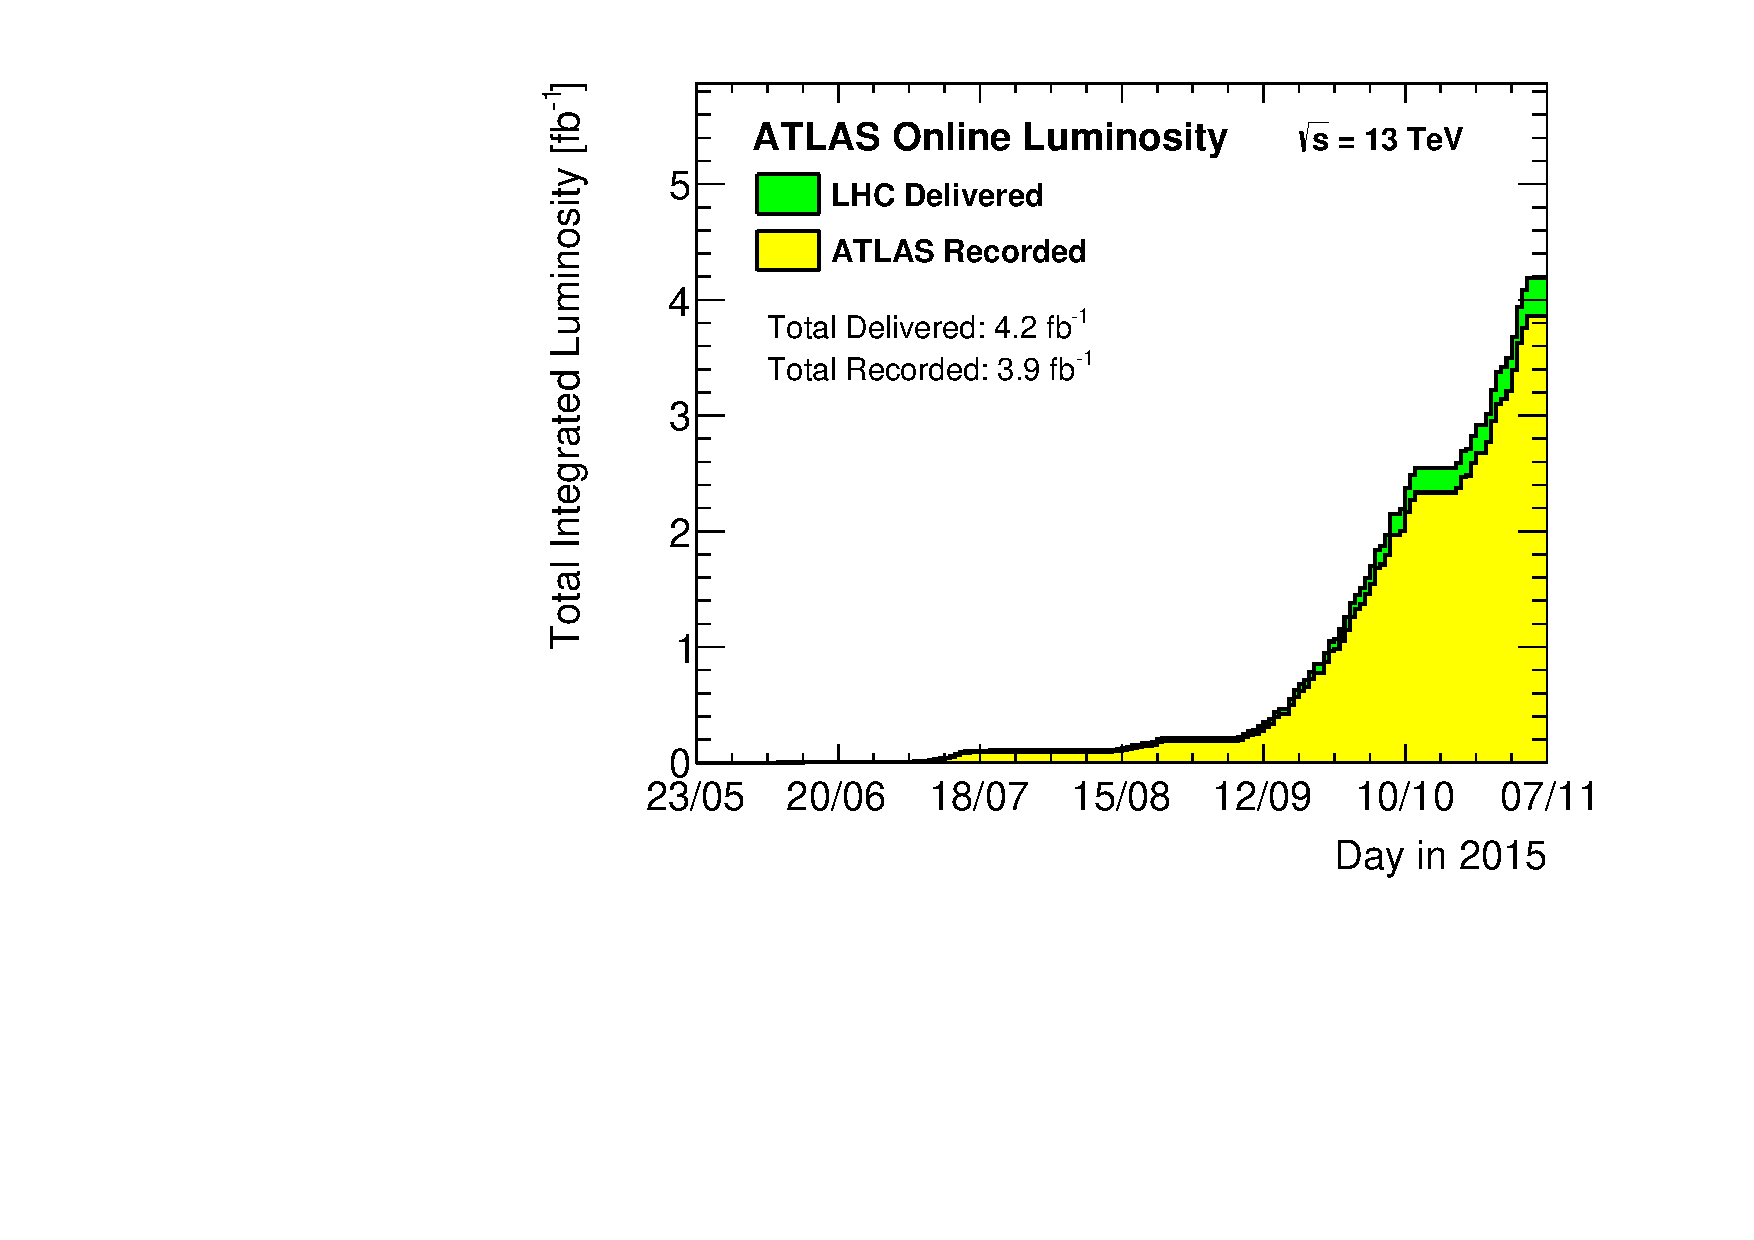
\includegraphics[width=0.45\linewidth, angle=0]{figs/Detector/lumi_2015.pdf}
    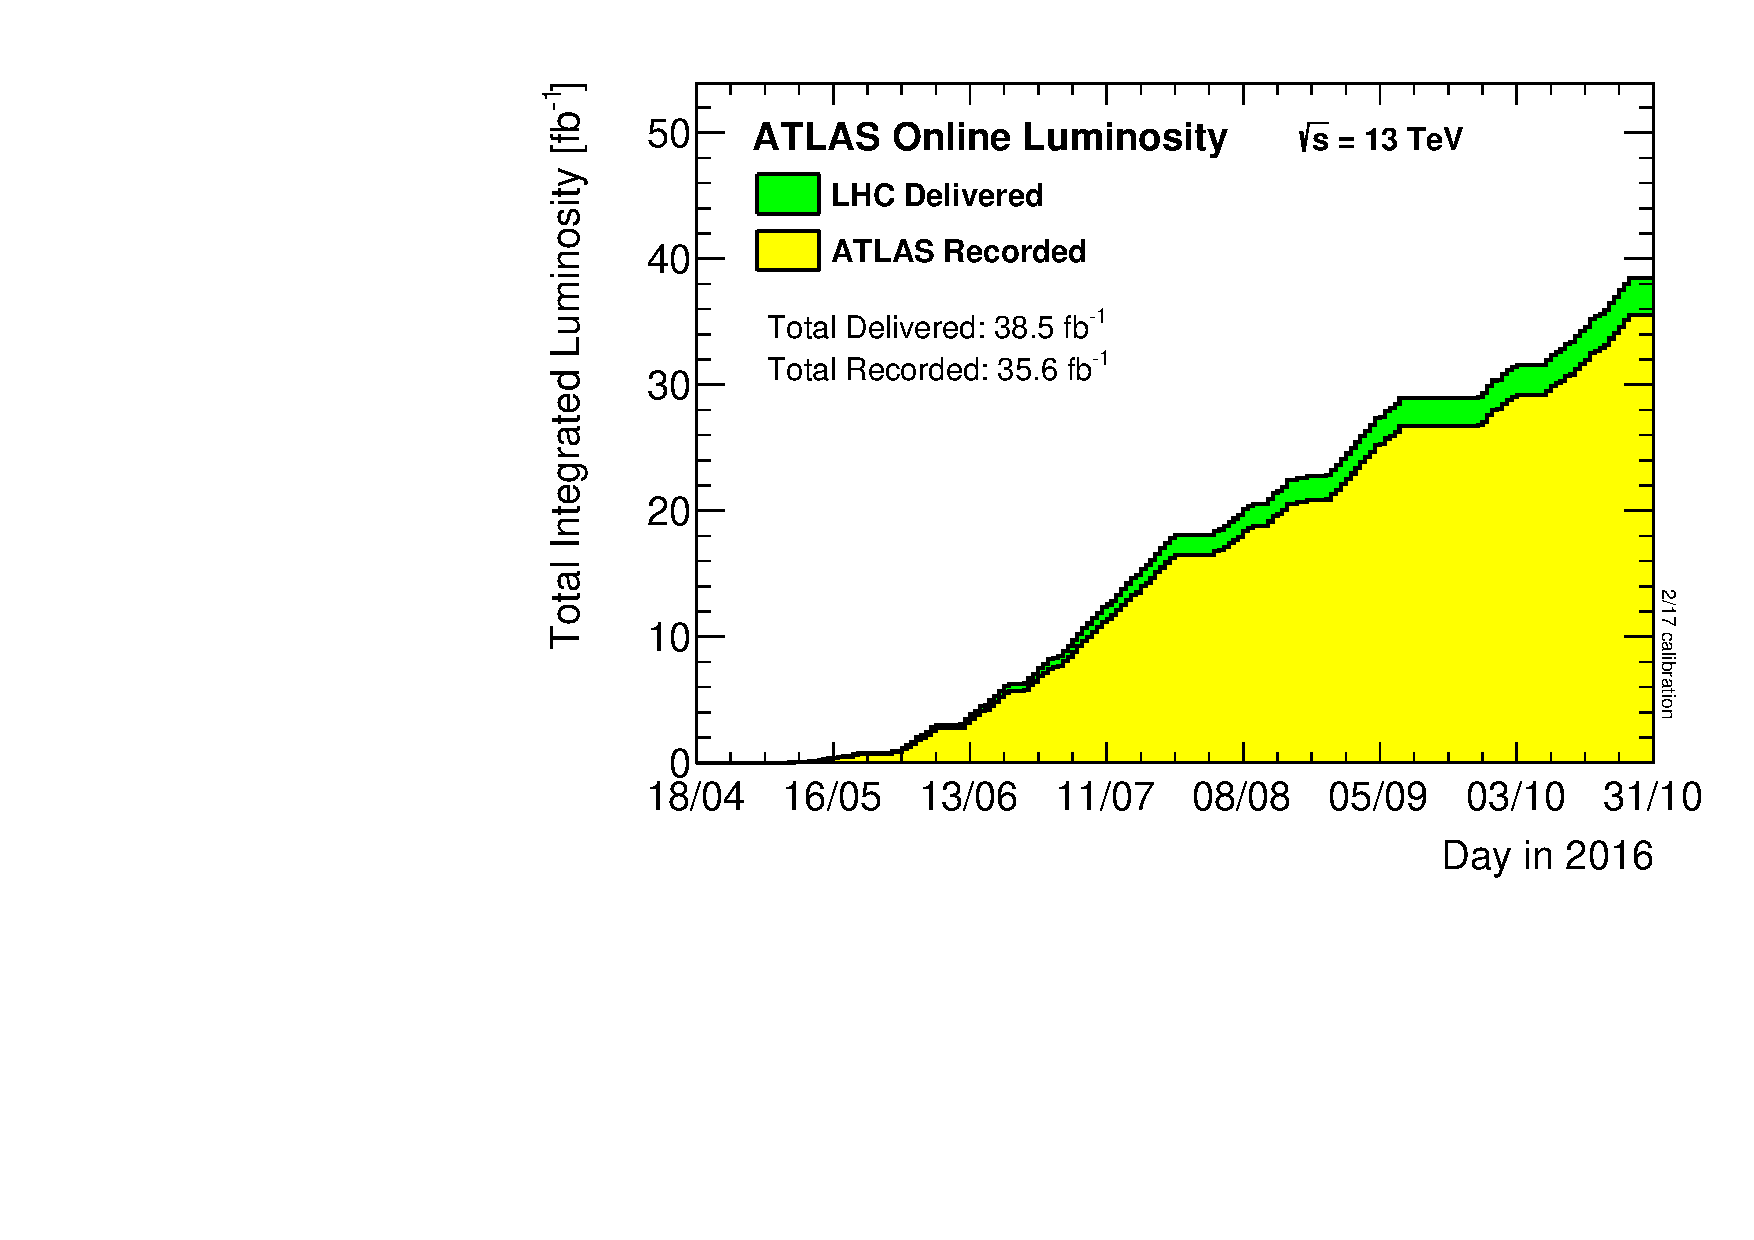
\includegraphics[width=0.45\linewidth, angle=0]{figs/Detector/lumi_2016.pdf}
  \end{center}
  \caption[Cumulative luminosity versus time delivered to (green) and recorded by ATLAS (yellow) during stable beams for pp collisions at 13 TeV centre-of-mass energy in (a) 2015 and (b) 2016]
      {Cumulative luminosity versus time delivered to (green) and recorded by ATLAS (yellow) during stable beams for pp collisions at 13 TeV centre-of-mass energy in (a) 2015 and (b) 2016~\cite{det-ATLAS_lumi_twiki}.}
  \label{fig:det-lumi_2015_2016}
\end{figure}

\section{ATLAS Detector Description}
\label{sec:det-ATLAS}

The ATLAS (\textbf{A} \textbf{T}oroidal \textbf{L}arge Hadron Collider \textbf{A}pparatu\textbf{S}) detector
design, construction and performance has been described in detail previously
\cite{det-ATLAS_Exp, det-ATLAS_TDR, det-ATLAS_Perf},
so what follows in this chapter is a general description of the detector with a focus on the
needs of the analysis that is being presented.
The ATLAS detector is effectively a large closed cylindrical detector,
made up of four key components which sit in concentric rings around the interaction point, where the proton bunches collide.
These components are the inner detector, calorimeters, muon spectrometer and the magnets; each of which are described in further detail below.
This design is used as each sub-detector measures different quantities and interacts differently to the various range of particles that ATLAS is required to observe,
meaning the ATLAS detector is able to identify and measure the key properties of particles that pass through its volume.
Figure~\ref{fig:det-ATLAS_schem} shows a cut-away schematic of the detector
and Figure~\ref{fig:det-ATLAS_slice} shows a slice of the detector in the plane perpendicular to the beam-pipe,
overlaid are simplified illustrations how the detector can respond to a range of particles~\cite{det-thesis_gutchow}.


\begin{figure}[!ht]
  \begin{center}
    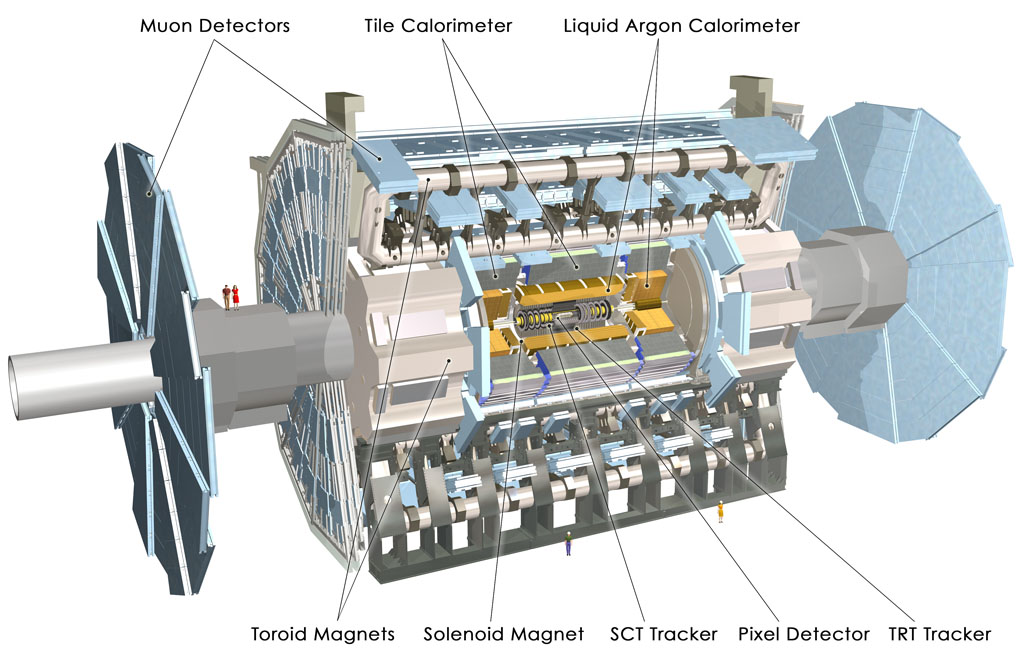
\includegraphics[width=1\linewidth, angle=0]{figs/Detector/ATLAS_schem.jpg}
  \end{center}
  \caption[A cut-away schematic of the ATLAS detector.]{ A cut-away schematic of the ATLAS detector~\cite{det-ATLAS_Exp}.}
  \label{fig:det-ATLAS_schem}
\end{figure}

\begin{figure}[!ht]
  \begin{center}
    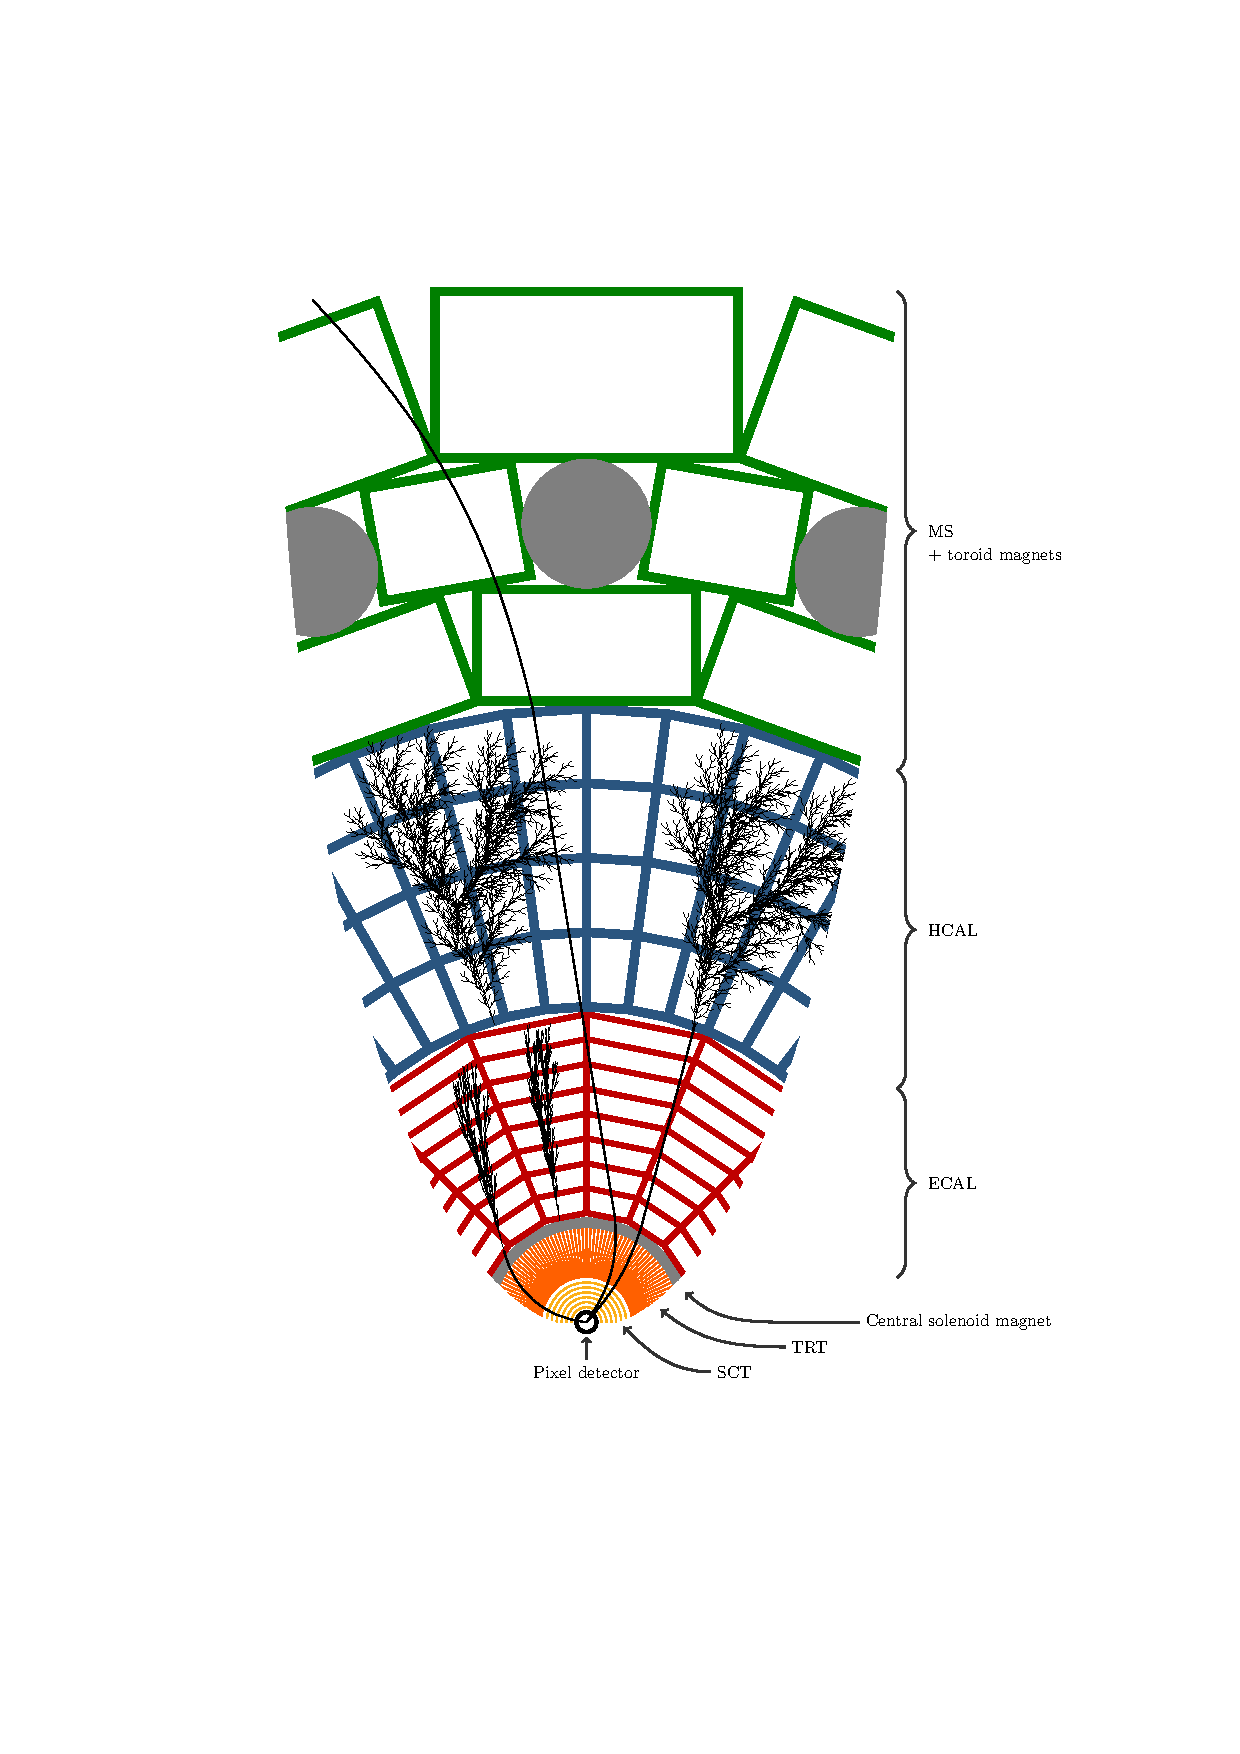
\includegraphics[width=1\linewidth, angle=0]{figs/Detector/ATLAS_slice.pdf}
  \end{center}
  %When citing in a caption, use this set-up
  \caption[A visualisation of the ATLAS detector and the various sub-detectors.
    The view is taken as a slice in a plane perpendicular to the beam-pipe,
    showing the radial range from the beam-pipe to the edge of the detector.
    Overlaid are simplified illustrations of how various types of particles interact with the ATLAS detector;
    specifically from left to right the particles are an electron, a chargeless hadron (e.g. a neutron), a photon, a muon and a charged hadron (e.g. proton).
    The sub-detector components are not to scale.]
          {A visualisation of the ATLAS detector and the various sub-detectors.
    The view is taken as a slice in a plane perpendicular to the beam-pipe,
    showing the radial range from the beam-pipe to the edge of the detector.
    Overlaid are simplified illustrations of how various types of particles interact with the ATLAS detector;
    specifically from left to right the particles are an electron, a chargeless hadron (e.g. a neutron), a photon, a muon and a charged hadron (e.g. proton).
    The sub-detector components are not to scale~\cite{det-thesis_gutchow}.}
  \label{fig:det-ATLAS_slice}
\end{figure}

\subsection{ATLAS Co-ordinate System}

Firstly, to describe the detail of the ATLAS detector there must be a description of the co-ordinate system that is used.
ATLAS uses a right-handed coordinate system, in which the origin lies at the interaction point.
The $x$-axis points to the centre of the LHC ring parallel to the surface of the earth,
the $y$-axis points towards the surface of the earth
and the $z$-axis runs along the beam-pipe, pointing anti-clockwise along the LHC beam-pipe.
The azimuthal angle, $\phi$, is defined right-handedly around the $z$-axis starting at the $x$-axis.
%Figure~\ref{fig:det_coordinate} illustrates this co-ordinate system.


The polar angle, $\theta$, is defined as the angle measured from the $z$-axis,
such that along the $z$-axis corresponds to $\theta = 0$
and anti-aligned with the $z$-axis corresponds to $\theta = \pi$.
However, to define the angular direction with respect to the z-axis the ATLAS co-ordinate system uses pseudo-rapidity, $\eta$, instead of using \theta, for reasons that will be outlined below.
$\eta$ is defined as a function of $\theta$:
\begin{equation}
 \eta = -\ln\left[\tan\left( \frac{\theta}{2} \right) \right]
\end{equation}
Thus, $\eta = 0$ corresponds to a particle travelling perpendicular to the beam-pipe,
where a positive value of $\eta$ corresponds to a particle travelling with a tilt towards the $z$-axis.
The quantity is called pseudo-rapidity as in the massless limit ($\lim_{E\to|\vec{p}|}$)
it can be shown that $\eta$ converges to rapidity, $y$, where rapidity is defined as,
\begin{equation}
  y = \frac{1}{2} \ln \left( \frac{E+p_{z}}{E-p_{z}} \right)
\end{equation}
A key property of rapidity is that the differences in rapidity, $\Delta y$, are invariant against Lorentz boosts along the $z$-axis.
Thus, $\eta$ is the final variable chosen in the ATLAS co-ordinate system due to the relation of $\eta$ with both $\theta$ and $y$
and the above mentioned property of $\Delta y$.
One final quantity commonly used within ATLAS is the variable $\Delta R$, which is defined as
\begin{equation}
  \Delta R = \sqrt{\Delta\eta^{2} + \Delta\phi^{2}}
\end{equation}
\Delta R represents an angular separation between two vectors within the ATLAS co-ordinate system.


Now that we have discussed the ATLAS co-ordinate system, we can provide a description of the components of the ATLAS detector.

\subsection{Inner Detector}
\label{sec:det-ID}

The Inner Detector (ID), the innermost sub-detector on ATLAS,
measures the trajectory of charged particles passing through the detector.
The ID is constructed from many concentric layers of detector,
and as a charged particle passes through the detector each of the layers provides a position measurement, known as a hit.
Then using the hits from the many layers the trajectory of the particle can be determined;
the measured trajectory is known as a track.
The ID is immersed in a 2~T magnetic field which bends the particle's trajectories;
from the sign and magnitude of the track's curvature the charge and momentum of the particle can be inferred.
The ID is made of three main component parts; the pixel detector, the Semi-Conductor Tracker
(SCT) and the Transition Radiation Tracker (TRT), as visualised in Figure~\ref{fig:det-ID_schem}.
The ID consists of the barrel, which are made up of cylinders surrounding the beam-pipe to cover low absolute values of $\eta$,
and the end-caps, which lie  perpendicular to beam-pipe on either end of the barrel to cover large values of absolute $\eta$:
here the description focuses on the barrel as this covers the $\eta$ range considered by the analysis.

\begin{figure}[!ht]
  \begin{center}
    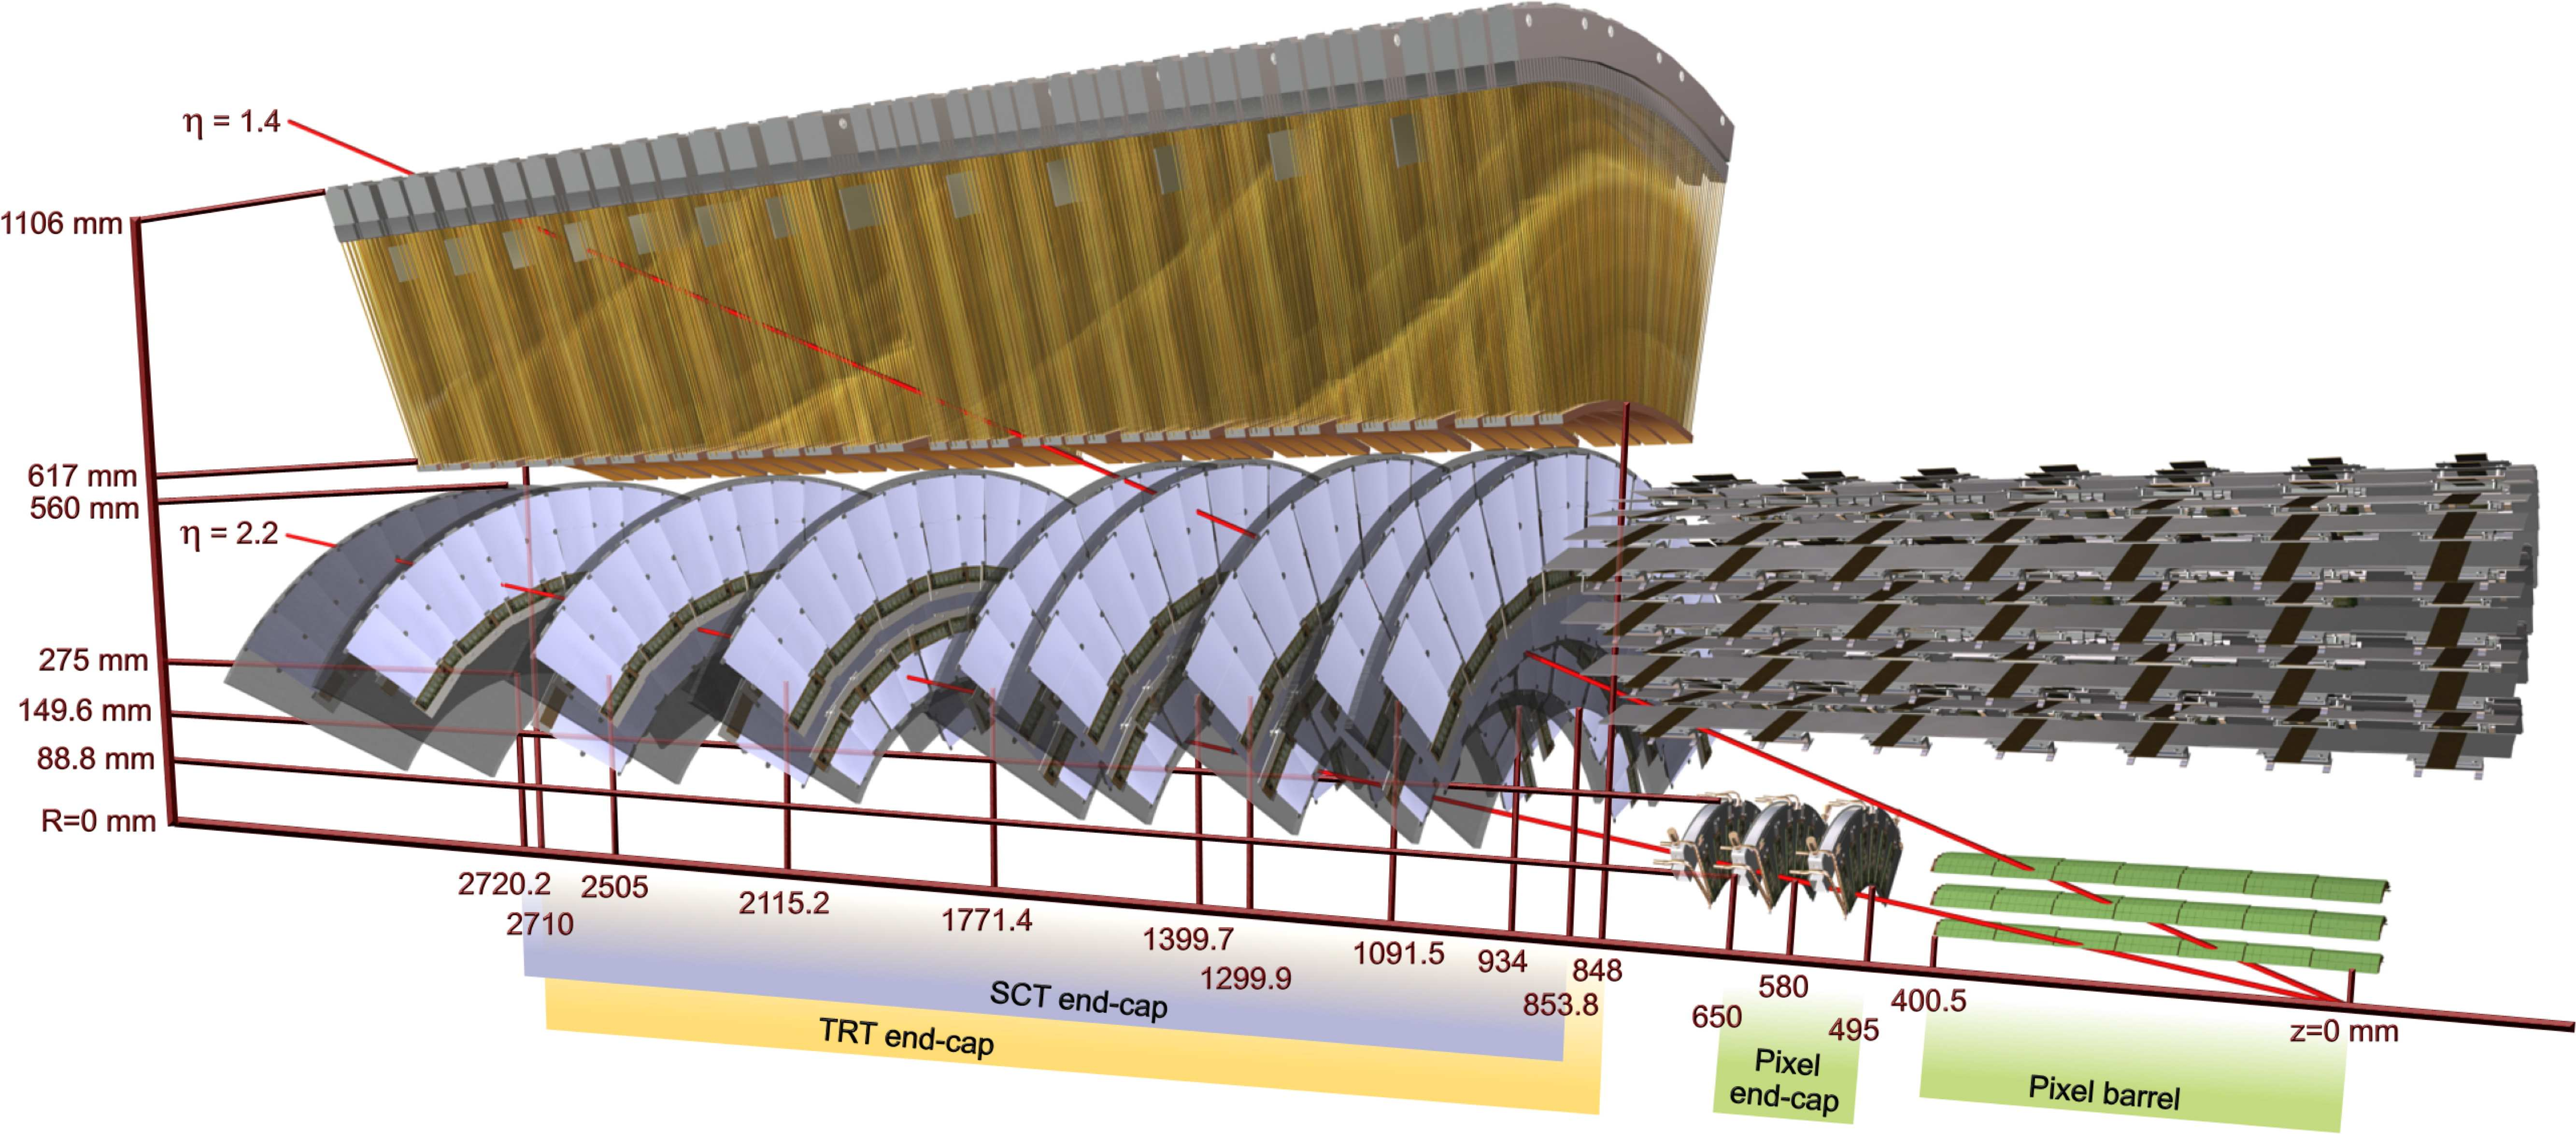
\includegraphics[width=0.8\linewidth, angle=0]{figs/Detector/ID_schem.pdf}
  \end{center}
  \caption[A cut-away schematic of the ATLAS Inner Detector (ID).]{A cut-away schematic of the ATLAS Inner Detector (ID)~\cite{det-ATLAS_Exp}.}
  \label{fig:det-ID_schem}
\end{figure}

The innermost component of the ID is the silicon pixel detector;
in the barrel this detector consists of 4 high-granularity layers of silicon based pixel modules surrounding the beam pipe,
covering a range of $-2.5 < \eta < 2.5$ and a radial distance of \SI{33}{mm} to \SI{122.5}{mm} \cite{det-IBL_TDR, det-IBL_Talk}.
The high-granularity of the pixel layers, allows for high precision measurements,
with an intrinsic resolution of approximately resolution of $\sim$\SI{10}{\micro\metre} in $R-\phi$ plane
and $\sim$\SI{115}{\micro\metre} in the z-direction. 

Moving radial outwards the next component of the ID is the Semi-Conductor Tracker;
which, in the barrel, comprises of 4 cylindrical layers of silicon micro-strips
covering a range of $-2.5 < \eta < 2.5$ and a radial distance of 299 mm to 514 mm.
The SCT has an intrinsic resolution of $\sim$\SI{17}{\micro\metre} in $R-\phi$ plane
and $\sim$\SI{580}{\micro\metre} in the z-direction. 

The outermost component of the ID is the Transition Radiation Tracker (TRT)
constructed of many \SI{4}{\mm} radius tubes filled with xenon.
As a charged particle passes through the gas,
it will cause ionisation allowing a measurement of its position using drift-time.
In the barrel, each tube provides a measurement in the $R-\phi$ plane
with an intrinsic resolution of ~\SI{130}{\micro\metre}
and the TRT will typically provide 36 hits per track.
In addition to a position measurement, due to the choice of the material between the tubes,
a particle passing through the detector will radiate photons
at an intensity inversely correlated to the mass of that particle,
providing additional information for particle identification. 

The trajectory, momentum and charge measurements provided by the Inner Detector are essential for particle identification in ATLAS.
In particular, the high precision measurements close to the beam-line allow for vertex reconstruction,
which is essential for identification of tracks coming from B or C hadrons, and hence the identification of $b$-jets.
This process, known as $b$-tagging, is discussed further in Section~\ref{sec:obj-bjets}\textit{(object definition and selection)}
and is important within the context of this analysis. 

\subsection{Calorimeters}
\label{sec:det-calo}

The ATLAS calorimeter, located on the outside of the magnet solenoid surrounding the ID,
is designed to provide an energy measurement of the traversing particles.
Accurate energy measurements are essential for a good resolution
of the mediator mass reconstructed from its decay products,
which is important within the context of the analysis being presented in this thesis.

The calorimeter at ATLAS is made up of two different systems that are built in concentric rings;
the inner-most is the Electromagnetic Calorimeter system (ECAL), which is used to measure electromagnetic objects such as photons and electrons.
Outside of that is the Hadronic Calorimeter system (HCAL), designed to provide an energy measurement of hadronic material.
The HCAL is built from the Tile and Hadronic Endcap calorimeters.
Both the ECAL and HCAL have barrel and end-cap components to make energy measurements at a large range of $\eta$ values.
Figure \ref{fig:det-calo_schem} shows a cut-away of the ATLAS calorimeter.

\begin{figure}[!ht]
  \begin{center}
    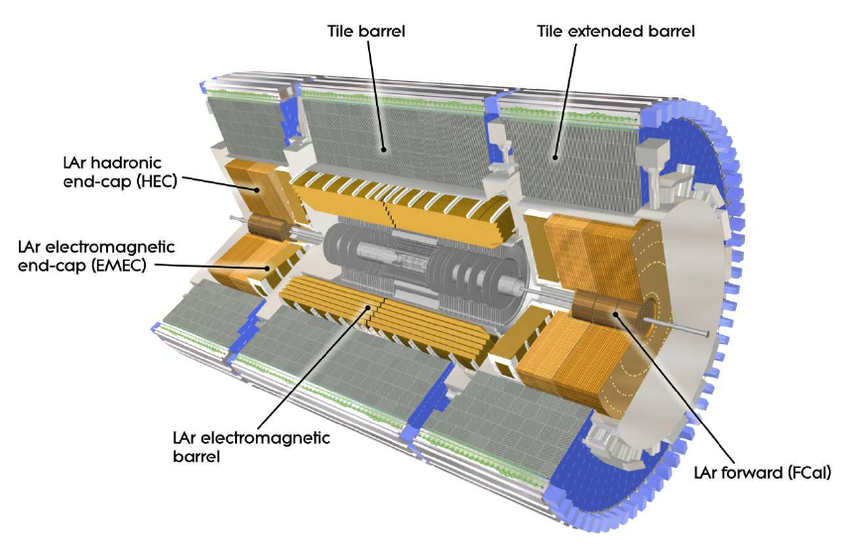
\includegraphics[width=1\linewidth, angle=0]{figs/Detector/Calo_schem.png}
  \end{center}
  \caption[A cut-away schematic of the ATLAS calorimeter system.]
          {A cut-away schematic of the ATLAS calorimeter system~\cite{det-ATLAS_Exp}.}
  \label{fig:det-calo_schem}
\end{figure}

Below I provide a more detailed description of the calorimeter components;
however, the principle behind each detector is common so is described first.
The calorimeters at ATLAS are sampling calorimeters, which means they consist of alternating layers of absorber and active material.
The role of the of the absorber layer is to force the particle, whose energy we want to measure, to emit secondary particles.
These secondary particles will again emit further particles and so on meaning a ``particle cascade'' is formed.
The role of the active material layer is to measure the energy of the many resulting particles from the cascade, known as the cascade particles.
The ATLAS detector is built such that the initial particle will cascade within the volume of the calorimeter system
and then, from a measurement of the energy of all the cascade particles,
the energy of the initial particle can be inferred. 

\subsubsection{Electromagnetic Calorimeter (ECAL)}

For the electromagnetic interaction, at energies $\sim \geq$\SI{1}{\GeV} the particle cascade process is mainly caused by two processes;
bremsstrahlung, ($e^{+/-} \to e^{+/-} + \gamma$) and pair production ($\gamma \to e^{+} + e^{-}$).
The electromagnetic calorimeter at ATLAS is known as the Liquid Argon (LAr) calorimeter.
The absorber material used in the LAr calorimeter is lead, due to its large density of charged particles (high Z)
which increases the rate of the cascade processes.
The active material is liquid argon;
when a cascade particle passes through the liquid argon it causes ionisation,
and the released electrons are captured using an electric field.
The number of released electrons is proportional to the energy of the cascade particle,
meaning that the energy of the cascade particle can be measured. 

As discussed above the LAr is split up into two sections;
the barrel section covers a region of $|\eta| < 1.475$ and two end-cap components cover $1.375 < |\eta| < 3.2$.
The depth of an electromagnetic calorimeter is often expressed in terms of the radiation length, $X_{0}$,
which is the distance that an electron's energy reduces by a factor of $e^{-1}$ through bremsstrahlung,
or 7/9 of the mean free path for a photon to pair produce electrons.
It is worth noting that this quantity is strongly material dependant;
a high-Z material, such as lead, has a shorter $X_0$.
The LAr calorimeter has a depth of $>$ 22 $X_{0}$ in the barrel and $>$ 24 $X_{0}$ in the end-caps,
meaning that almost all of the particle shower from a high-energy photon
or electron can be contained within electromagnetic calorimeter. 

\subsubsection{Hadronic Calorimeter (HCAL)}

If a particle can also interact through strong interactions, such as the components of a hadronic jet,
then the particle cascade is a more complicated process.
A hadronic cascade processes is dominated by processes such as
ionisation, nuclear spallation and neutron generation \cite{det-nuclearInt_book, det-thesis_kate}.
For a chargeless hadron, for example a neutron,
strong processes, such as spallation, are the only processes that contribute to its cascade.
During these hadronic cascade processes many $\pi_0$ mesons are made,
which can decay to a pair of photons and thus form electromagnetic cascade as described above. 

For hadronic interactions, the size of detector is measured by the interaction length, $\lambda$,
defined as the distance required to reduce the number of relativistic hadrons by $e^{-1}$.
This means that by the end of the LAr calorimeter there is 2.3 $\lambda$ of active material in the barrel,
so the full hadronic shower cannot be captured by the LAr calorimeter alone.
For a full measurement of the hadronic energy, the Hadronic Calorimeter system (HCAL) is required. 

The Tile Calorimeter is constructed from absorber layers of steel and active material layers of scintillating tiles,
and has a depth of 7.4 $\lambda$, meaning the majority of the hadronic shower can be captured by either the LAr calorimeter or the Tile calorimeter.
The Tile Calorimeter is split up into the barrel and the extended barrel components;
the barrel covers the region $|\eta| <$ 1.0 and the extended barrel covers the region $0.8 < |\eta| < 1.7$. 

To cover the more forward regions there are two more calorimeter detectors.
The Hadronic Endcap Calorimeter (HEC) is housed in two large wheels at either end of the ATLAS detector
and covers a region of $1.5 < ∣\eta∣ < 3.2$.
The HEC is a sampling calorimeter built using copper as the absorber layers and liquid argon as the active material
and has a depth of $\sim 12~\lambda$.
In addition the Forward Calorimeter (FCAL) covers the very forward region of $3.1 < ∣\eta∣ < 4.9$,
which is outside the range considered within this analysis.
It is constructed from absorber layers of
copper (for EM interactions)
and tungsten (for hadronic interactions)
with liquid argon for the active material layers. 

Another important point about the ATLAS calorimeter is that it is non-compensating calorimeter;
that is to say that the response of the detector to an electromagnetic particle (such as an electron)
is larger than the response of a hadronic particle (for example a pion).
The reason for this is some energy is lost in hadronic cascade process;
mainly due to the energy required to release nucleons from calorimeter nuclei during spallation,
but also from the recoil energy given to the calorimeter nuclei
and neutrinos created during strong processes that can escape the calorimeter \cite{det-comp_calo, det-thesis_lene}.
To account for the fact that the ATLAS calorimeter is non-compensation,
calorimeters are calibrated to the EM-scale
and then a jet energy scale correction is applied,
this process is described further in Section~\ref{sec:obj-jets}\textit{(object definition and selection)}. 

\subsection{Muon Spectrometer}
\label{sec:det-MS}

The only standard model particle visible to ATLAS which can pass through the calorimeter is the muon;
hence to identify and obtain the momentum of muons an additional detector, the Muon Spectrometer (MS), is used.
The MS is a detector which surrounds the hadronic calorimeter,
measuring the momentum of muons by observing the curvature of their trajectories in magnetic fields.
Trajectories are determined using muon position measurements from multiple layers of detectors,
analogous to what has been described for the inner detector. 

In the barrel region ($|\eta| < 1.4$) the large barrel toroid provides the magnetic field,
in the end-cap region ($1.6 < |\eta| < 2.7$) the two smaller end-cap magnets  provide the magnetic field
and finally in the transition region ($1.4 < |\eta| < 1.6$) both sets of magnets contribute to the magnetic field.
A further description of the magnets used in ATLAS is found in the next section. 

Muon chambers are the detectors tasked with providing the muon position measurements required to reconstruct muon tracks.
The muon chambers come in two types; trigger and precision.
The trigger muon chambers provide a quick position measurement in 3-dimensions which can be used
to identify muons tracks in the trigger.
The trigger muon chambers cover a range $|\eta| < 2.0$;
consisting of Resistive Plate Chambers (RPC’s) in the barrel and Thin Gap Chambers (TGC’s) in the end-cap regions.
The precision muon chambers provide a precise measurement of the muon position co-ordinates in the $R-z$ plane,
the plane in which track curvature occurs in the muon spectrometer, allowing for precise measurements of the muon track-$p_T$. 
In the barrel region, precision muon chambers are arranged in three concentric cylindrical layers of chambers formed around the beam-pipe,
whilst in the transition and end-cap regions there are three layers of chambers either side of the barrel lying in disks perpendicular to the beam-pipe.
In the region $|\eta| < 2.0$, the precision muon chambers are made from Monitored Drift Tubes (MDTs),
whilst at large pseudo-rapidities ($2.0 < |\eta| < 2.7$), Cathode Strip Chambers (CSCs) are used.


There is an additional use of the muon spectrometer that relates to high-energy jets.
Whilst for most jets their shower is fully contained within the calorimeter
there are some jets, particularly at high-$p_T$, where a non-negligible fraction of energy from the shower goes beyond the calorimeter.
This effect, known as `punch-through', is accounted for using energy deposits in the muon spectrometer.

\subsection{Magnets}
\label{sec:det-magnets}

\begin{figure}[!ht]
  \begin{center}
    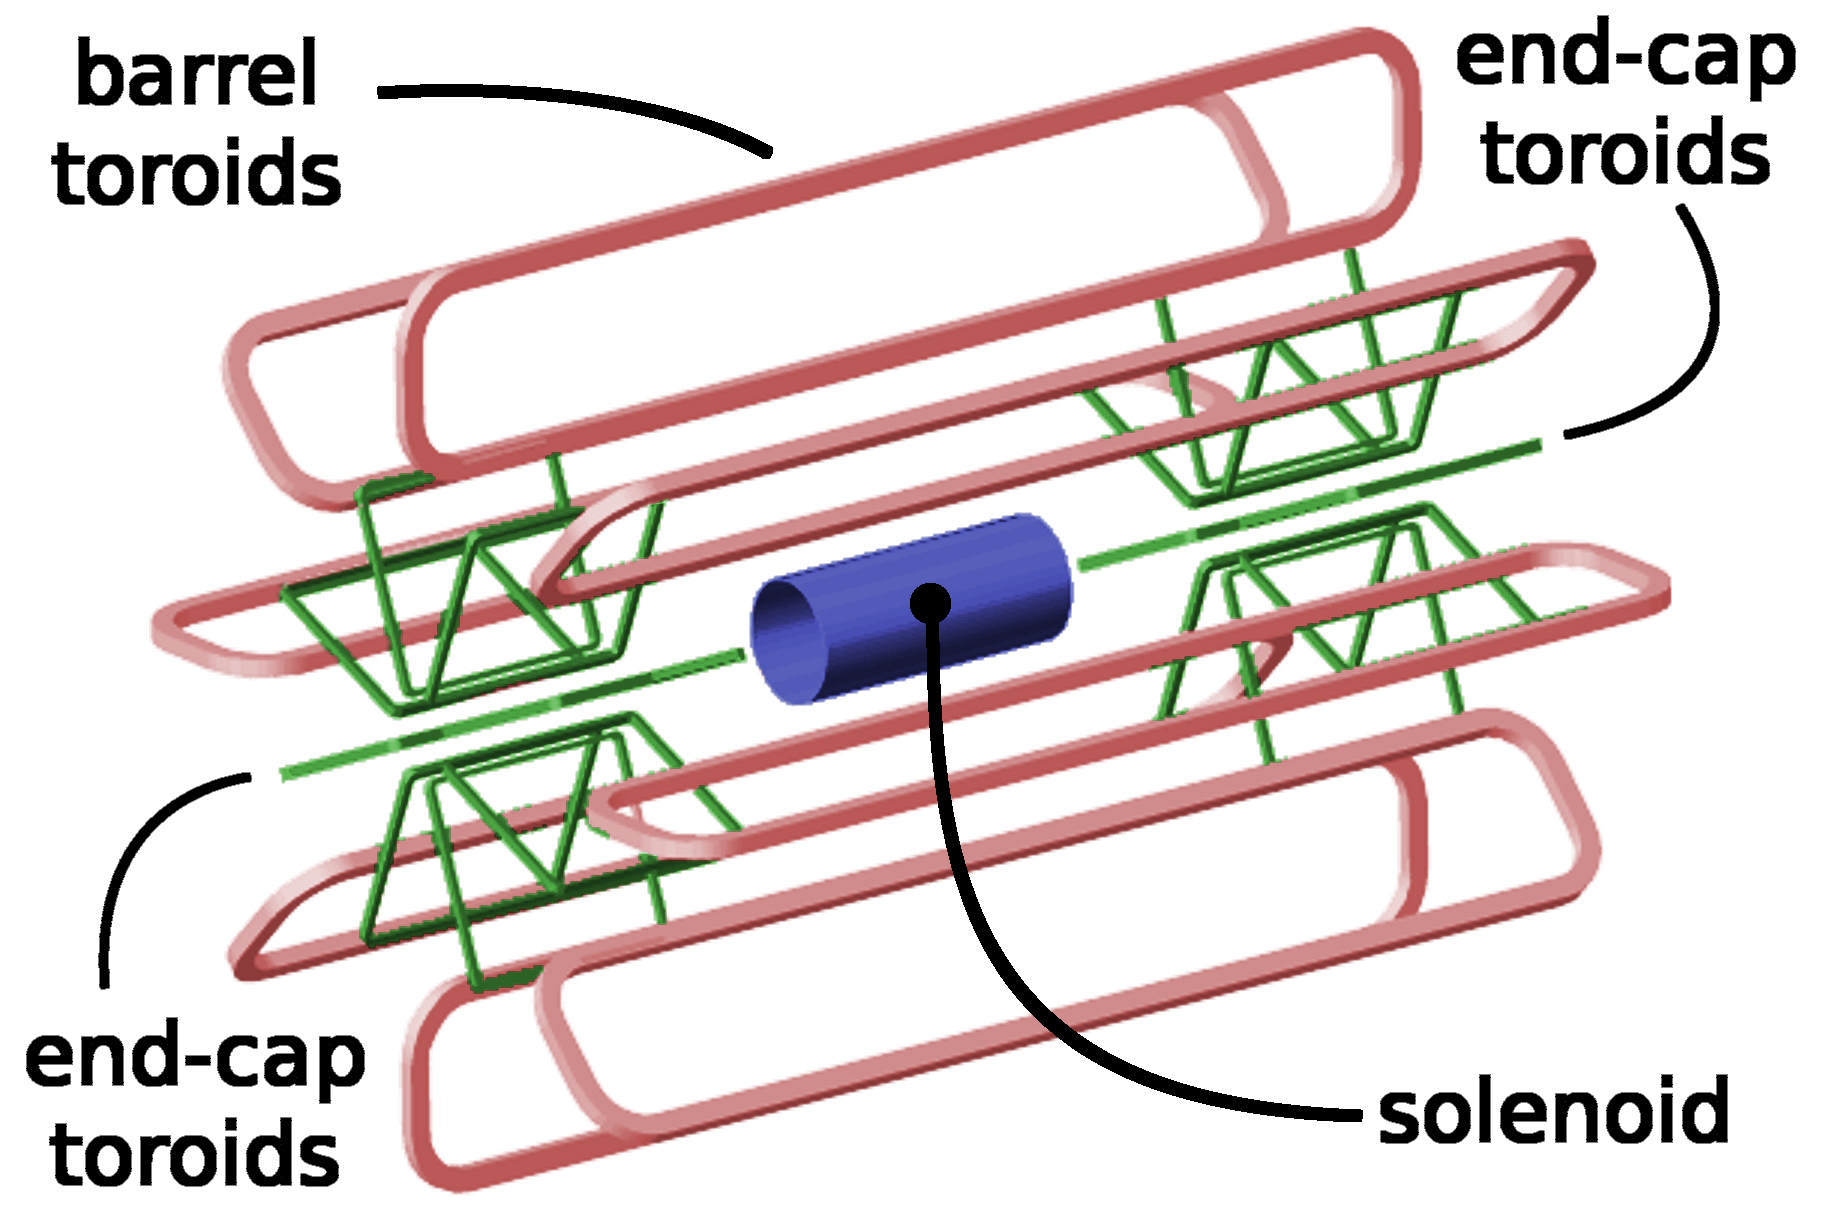
\includegraphics[width=1\linewidth, angle=0]{figs/Detector/Magnet_schem.png}
  \end{center}
  \caption[The layout of the ATLAS magnets.]{The layout of the ATLAS magnets~\cite{det-magnet_fig}.}
  \label{fig:det-magnet_schem}
\end{figure}


In ATLAS magnetic fields are important for obtaining the momentum and charge of particles from their observed trajectories in the ID and Muon Spectrometer.
ATLAS is made up of four large superconducting magnets;
the inner solenoid which surrounds the inner detector and provides a 2~T magnetic field within the ID.
The barrel toroid magnet provides a magnetic field of up to 2.5~T in the central regions of the muon spectrometer and
the two end-cap toroid magnets which produce a magnetic field of up to 3.5~T in the forward regions of the MS.
Figure~\ref{fig:det-magnet_schem} shows the layout of the magnets in ATLAS \cite{det-magnet_fig}.

%\section{Data Acquisition and Trigger}
\section{Trigger}
\label{sec:det-trig}

In 2015 and 2016, the LHC has been colliding proton beams with a spacing of \SI{25}{\nano\second},
meaning that the ATLAS experiment has been taking data at a rate of 40 MHz.
However, due to the large computing resources required to process and store each event,
it is not possible to record all this data for use in an analysis.
To resolve this problem,
the ATLAS experiment uses a trigger system to reduce the event rate by
selecting the events of interest that contain high-$p_{T}$
%$\footnote{$p_{T}$ refers to the component of momentum transverse to the beam-line.} 
physics objects, which indicate that a hard scatter has occurred in that event. 

The ATLAS trigger-system has two levels;
the first level trigger (L1) and the higher level trigger (HLT) \cite{det-run2_trigger}.
Figure~\ref{fig:det-trigger_schem} shows a schematic outlining the trigger used in Run-2 \cite{det-run2_triggerPerf}. 

\begin{figure}[!ht]
  \begin{center}
    \includegraphics[width=1\linewidth, angle=0]{figs/Detector/trigger_schem.png}
  \end{center}
  \caption[A schematic of the ATLAS trigger and data-acquisition system in Run-2, with a focus on the components required for triggering.]
          {A schematic of the ATLAS trigger and data-acquisition system in Run-2, with a focus on the components required for triggering~\cite{det-run2_trigger}.}
  \label{fig:det-trigger_schem}
\end{figure}

The first level trigger (L1) is hardware based which reduces the rate from 40~MHz to 100~kHz within a time window of \SI{2.2}{\micro\second}.
The L1 trigger uses custom electronics to rapidly process information directly from the
calorimeter and the muon spectrometer, searching for high-$p_{T}$ muon tracks and large calorimeter deposits.
The information is then passed to the central trigger which uses a set of pre-defined conditions
to decide if a L1 trigger accept is given and thus events are passed on to the next step of triggering.
At the same time Regions of Interests (ROIs) are constructed around the objects that have fired the L1 trigger,
which are passed on to the HLT. 

The next step is the HLT, a software based trigger,
which further reduces the event rate to 1~kHz within a time window of ~\SI{0.2}{\second}.
The HLT uses the information from the full detector
to perform a more complete reconstruction of the physics objects within the event,
the most time consuming reconstruction algorithms only being run only within the ROIs taken from L1.
The more complex event analysis allowed within the software-based trigger includes
track reconstruction and therefore allows for $b$-jet identification.
If the content of the event reconstruction passes a pre-set criteria, a HLT accept is issued
meaning that the events are passed on for processing and storage. 
% in offline computer farms (known as tier-0). 

A further description of triggers used in the analysis,
with a particular focus on the $b$-jet trigger performance
can be found in \ref{sec:bJetTrigger}\textit{(b-jet trigger chapter)}.

